\section{Задача №3}

\subsection{Формулировка задачи}

\indent

Решить задачу Дирихле для уравнения Лапласа в прямоугольнике $l_{1}\times l_{2}$, когда на верхней границе задан поток $\frac{\partial u(x, l_{2})}{\partial y} = \sin \left( \frac{\pi x}{l_{1}} \right)$, а на остальных границах заданы нулевые значения функции.

\subsection{Постановка задачи}

\begin{wrapfigure}{r}{0.25\textwidth}
    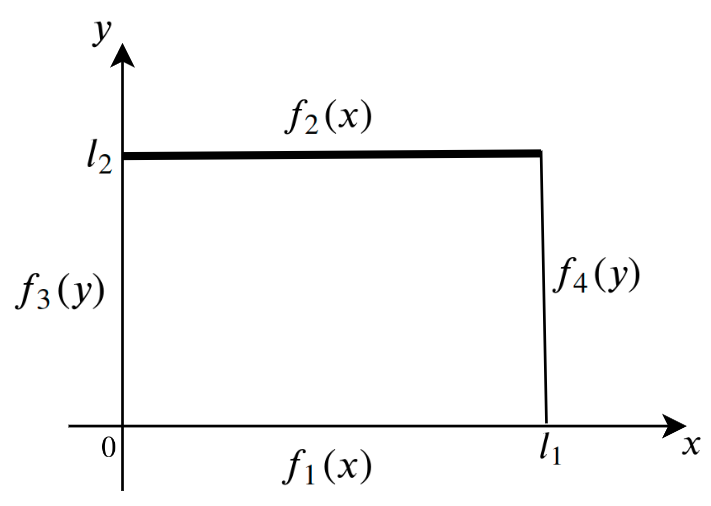
\includegraphics[width=0.34\textwidth]{task3_source.png}
\end{wrapfigure}
\leavevmode

\setcounter{equation}{0}

\begin{numcases}{}
\Delta u = 0\,\,\,\text{- условие Лапласа}, &\text{$0 < x < l_{1}; 0 < y < l_{2};$}\\
u(x, 0) = f_{1}(x) = 0;\\
u_{y}(x, l_{2}) = f_{2}(x) = \sin \left( \frac{\pi x}{l_{1}} \right);\\
u(0, y) = f_{3}(y) = 0;\\
u(l_{1}, y) = f_{4}(y) = 0
\end{numcases}
$\linebreak\linebreak\linebreak$

\subsection{Теоретические сведения}

\indent

При решении первой краевой задачи для прямоугольника требуется найти функцию $u$, удовлетворяющую уравнению (1) и граничным условиям (2)-(5) на границах прямоугольника.

Решим задачу методом разделения переменных, найдя частное решение уравнения (1) вида $u(x, y) = X(x)\cdot Y(y) \not\equiv 0$.

Подставляя это решение в оператор Лапласа: $X''Y + Y''X = 0$, получим:

$$\frac{X''}{X} = - \frac{Y''}{Y} = - \lambda^{2}\,\,\, \text{(задача Штурма-Лиувилля), где}\,\,\, \lambda = const.$$

Для нахождения функции $X$ получим уравнение второго порядка: $\frac{X''}{X} = -\lambda^{2}$, чтобы функция $u$ удовлетворяла нужному из условий, функция $X$ должна удовлетворять условиям: $X(a) = X(0) = 0$.

Далее задача решается совершенно обычным способом, а её общее решение этой задачи - функцию $u(x, y)$ можем искать в виде суммы основных решений.

\pagebreak

\subsection{Решение задачи}

\indent

Решим задачу методом разделения переменных: $u(x, y) = X(x) \cdot Y(y)$. Подставим в оператор Лапласа: $X''Y + Y''X = 0$

$$\frac{X''}{X} = -\frac{Y''}{Y} = -\lambda^{2}$$

В решении уравнения теплопроводности при $\lambda^{2} \geq 0$ решений нет.

\begin{equation*}
\begin{aligned}
\text{Рассмотрим}\,\,\, \lambda^{2} < 0: \\
\end{aligned}
\quad \left\{
\begin{aligned}
       & X'' + \lambda^{2}X = 0; \\
       & X = C_{1} \sin{\lambda x} + C_{2} \cos{\lambda x}
\end{aligned}
\right.
\end{equation*}  

Из граничных условий (4), (5) получим:

\begin{equation*}
  \begin{split}
    X(0) & = C_{2} = 0;\\
    X(l_{1}) & = C_{1} \sin{\lambda l_{1}} = 0;
  \end{split}
\quad\rightarrow\quad
  \begin{split}
    & \sin{\lambda l_{1}} = 0;\\
    & \lambda l_{1} = \pi n, \quad n=1,2,3\ldots
  \end{split}
\end{equation*}

\begin{equation*}
  \begin{split}
    \boxed{\lambda_{n} = \frac{\pi n}{l_{1}}}
  \end{split}
\quad\quad
  \begin{split}
    \boxed{X_{n}(x) = \sin{\frac{\pi n}{l_{1}}x}}
  \end{split}
\quad\quad
\end{equation*}

Найдём $Y(y)$:

\begin{equation*}
  \begin{split}
    - \frac{Y''}{Y} = \lambda^{2}
  \end{split}
\Rightarrow
  \begin{split}
  	& Y'' - \lambda^{2}Y = 0;\\
  	& Y = A_{n} \cdot e^{-\frac{\pi n}{l_{1}}y} + B_{n} \cdot e^{\frac{\pi n}{l_{1}}y}
  \end{split}
\end{equation*}

$$u(x, y) = \sum_{n=1}^{\infty} \sin{\frac{\pi n}{l_{1}}x}\cdot \left( A_{n}\cdot e^{-\frac{\pi n}{l_{1}}y} + B_{n} \cdot e^{\frac{\pi n}{l_{1}}y} \right)$$

Подставим в краевые условия:

$$u(x, 0) = \sum_{n=1}^{\infty} (A_{n} + B_{n}) \cdot \sin{\frac{\pi n}{l_{1}}x} = 0 \Rightarrow A_{n} + B_{n} = 0$$

$$u_{y}(x, l_{2}) = \sum_{n=1}^{\infty} \left( -\frac{\pi n}{l_{1}} A_{n} \cdot e^{-\frac{\pi n}{l_{1}}l_{2}} + \frac{\pi n}{l_{1}} B_{n} \cdot e^{\frac{\pi n}{l_{1}}l_{2}} \right) \cdot \sin{\frac{\pi n}{l_{1}}x} \stackrel{\left(\lambda_{n} = \frac{\pi n}{l_{1}} \right)}{=} \sin{\frac{\pi x}{l_{1}}} \Rightarrow$$

\begin{multline*}
    \quad\quad\quad\quad\quad\quad\quad\Rightarrow \lambda_{n} = \frac{\pi}{l_{1}} \Rightarrow n = 1, \quad\quad \left( -\frac{\pi}{l_{1}} \right) \cdot A_{1} \cdot e^{-\frac{\pi}{l_{1}}l_{2}} + \left( \frac{\pi}{l_{1}} \right) \cdot B_{1} \cdot e^{\frac{\pi}{l_{1}}l_{2}} = 1, \\
    \left( -\frac{\pi n}{l_{1}} \right) \cdot A_{n} \cdot e^{-\frac{\pi n}{l_{1}}l_{2}} + \left( \frac{\pi n}{l_{1}} \right) \cdot B_{n} \cdot e^{\frac{\pi n}{l_{1}}l_{2}} = 0
\end{multline*}

Разобьём на две системы:

\begin{equation*}
  \circled{I}\!\!
  \begin{split}
    \begin{cases}
      A_{1} + B_{1} = 0;\\
      -\lambda_{1} \cdot A_{1} \cdot e^{-\lambda_{1}l_{2}} + \lambda_{1} \cdot B_{1} \cdot e^{\lambda_{1}l_{2}} = 1
    \end{cases}
  \end{split}
\quad\quad\circled{II}\,\,
  \begin{split}
    \begin{cases}
      A_{n} + B_{n} = 0;\\
      -\lambda_{n} \cdot A_{n} \cdot e^{-\lambda_{n}l_{2}} + \lambda_{n} \cdot B_{n} \cdot e^{\lambda_{n}l_{2}} = 0
    \end{cases}
  \end{split}
\end{equation*}

\circled{II} имеет единственное решение, поскольку:
$\begin{vmatrix}
A_{n}& B_{n}\\
-\lambda_{n}A_{n}e^{-\lambda_{n}l_{2}}& \lambda_{n}B_{n}e^{\lambda_{n}l_{2}}
\end{vmatrix}$
$\neq 0$, а это значит $A_{n} = B_{n} = 0$.

Решим систему \circled{I}:

$$
\begin{cases}
  A_{1} + B_{1} = 0;\\
  -\frac{\pi}{l_{1}} \cdot A_{1} \cdot e^{-\frac{\pi}{l_{1}}l_{2}} + \frac{\pi}{l_{1}} \cdot B_{1} \cdot e^{\frac{\pi}{l_{1}}l_{2}} = 1
\end{cases}
$$

Применим правило Крамера: 
$\Delta = 
\begin{vmatrix}
1& 1\\
-\frac{\pi}{l_{1}} \cdot e^{-\frac{\pi}{l_{1}}l_{2}}& \frac{\pi}{l_{1}} \cdot e^{\frac{\pi}{l_{1}}l_{2}}
\end{vmatrix}
= \frac{\pi}{l_{1}}\left( e^{\frac{\pi}{l_{1}}l_{2}} + e^{-\frac{\pi}{l_{1}}l_{2}} \right)$

\begin{equation*}
  \begin{split}
    \Delta_{1} = 
    \begin{vmatrix}
    0& 1\\
    1& \frac{\pi}{l_{1}} e^{\frac{\pi}{l_{1}}l_{2}}
    \end{vmatrix}
  \end{split}
= -1; \quad\quad \Delta_{2} =
  \begin{split}
    \begin{vmatrix}
    1& 0\\
    -\frac{\pi}{l_{1}} e^{-\frac{\pi}{l_{1}}l_{2}}& 1
    \end{vmatrix}
  \end{split}
= 1
\end{equation*}

\begin{equation*}
  \begin{split}
    A_{1} = \frac{\Delta_{1}}{\Delta} =
    \frac{-1}{\frac{\pi}{l_{1}}\left( e^{\frac{\pi}{l_{1}}l_{2}} + e^{-\frac{\pi}{l_{1}}l_{2}} \right)};
  \end{split}
\quad\quad
  \begin{split}
  B_{1} = \frac{\Delta_{2}}{\Delta} =
    \frac{1}{\frac{\pi}{l_{1}}\left( e^{\frac{\pi}{l_{1}}l_{2}} + e^{-\frac{\pi}{l_{1}}l_{2}} \right)}
  \end{split}
\end{equation*}

Подставим в $u(x, y)$:\,\,$\boxed {\sin{\frac{\pi}{l_{1}}x}\cdot \frac{1}{\frac{\pi}{l_{1}}\left( e^{\frac{\pi}{l_{1}}l_{2}} + e^{-\frac{\pi}{l_{1}}l_{2}} \right)} \cdot \left( -e^{-\frac{\pi}{l_{1}}y} + e^{\frac{\pi}{l_{1}}y} \right) = u(x, y)}$

$\linebreak$

\textbf{Проверка:} $u(x, 0) = \sin{\frac{\pi}{l_{1}}x} \cdot \cancelto{0}{\frac{(-1 + 1)}{\frac{\pi}{l_{1}}\left( e^{\frac{\pi}{l_{1}}l_{2}} + e^{-\frac{\pi}{l_{1}}l_{2}} \right)}} = 0$

$$ u_{y}(x, l_{2}) = \sin{\frac{\pi}{l_{1}}x}\cdot \cancelto{1}{\frac{1}{\frac{\pi}{l_{1}}\left( e^{\frac{\pi}{l_{1}}l_{2}} + e^{-\frac{\pi}{l_{1}}l_{2}} \right)} \cdot \left( \frac{\pi}{l_{1}}\cdot e^{-\frac{\pi}{l_{1}}l_{2}} + \frac{\pi}{l_{1}}\cdot e^{\frac{\pi}{l_{1}}l_{2}} \right)} = \sin{\frac{\pi}{l_{1}}x} $$

\begin{equation*}
  \begin{split}
    u(0, y) = \sin{0} \cdot \ldots = 0;
  \end{split}
\quad\quad
  \begin{split}
    u(l_{1}, y) = \sin \frac{\pi \not{l_{1}}}{\not{l_{1}}} \cdot \ldots = 0,\quad \text{получили верные равенства.}
  \end{split}
\end{equation*}

Ответ: $u(x, y) = \sin{\frac{\pi}{l_{1}}x} \cdot \frac{\left( -e^{-\frac{\pi}{l_{1}}y} + e^{\frac{\pi}{l_{1}}y} \right)}{\frac{\pi}{l_{1}}\left( e^{\frac{\pi}{l_{1}}l_{2}} + e^{-\frac{\pi}{l_{1}}l_{2}} \right)}$

\pagebreak

Построим график функции $u(x, y)$:

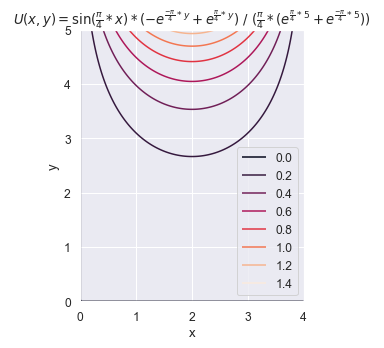
\includegraphics[width=0.8\linewidth]{Dirihle.PNG}

Из этой картины можно увидеть, что решение данной задачи было найдено верно, поскольку на верхней границе прямоугольника $l_{1}\times l_{2}$ происходит изменение потока, а на остальных границах - ничего, что полностью удовлетворяет поставленной задаче.

\pagebreak